% Created 2019-07-16 Tue 17:15
\documentclass[a4paper,twocolumn]{article}
\usepackage[utf8]{inputenc}
\usepackage[T1]{fontenc}
\usepackage{fixltx2e}
\usepackage{graphicx}
\usepackage{longtable}
\usepackage{float}
\usepackage{wrapfig}
\usepackage{rotating}
\usepackage[normalem]{ulem}
\usepackage{amsmath}
\usepackage{textcomp}
\usepackage{marvosym}
\usepackage{wasysym}
\usepackage{amssymb}
\usepackage{hyperref}
\tolerance=1000
\usepackage[citestyle=authoryear-icomp,bibstyle=authoryear,hyperref=true,backref=true,maxcitenames=3,url=true,backend=biber,natbib=true]{biblatex}
\addbibresource{BNNConsistency.bib}
\graphicspath{ {images/}}
\usepackage{subfig}
\setcounter{secnumdepth}{2}
\author{Sharan Yalburgi, Julyan Arbel}
\date{July, 2019}
\title{Studying Uncertainity in Bayesian Neural Networks}
\hypersetup{
  pdfkeywords={},
  pdfsubject={},
  pdfcreator={Emacs 25.2.2 (Org mode 8.2.10)}}
\begin{document}

\maketitle


\section{Abstract}
\label{sec-1}
Availability of uncertainity measure is the one of the major reasons why Bayesian Neural Networks are topics of interest. It is therefore essential to understand the behavior of these uncertainity measures with varying prior conditions, amount of data and modelling tasks.


\section{Introduction}
\label{sec-2}

Contributions of this paper is as follows:

\section{Previous Work}
\label{sec-3}

\subsection{Study of Bayesian Neural Networks with Non-Smooth Functions \cite{NNnonsmooth}}
\label{sec-3-1}

\subsection{Consistency of Posterior Distributions for Neural Networks \cite{lee2000consistency}}
\label{sec-3-2}

\subsection{Classification kwith imperfect training labels \cite{cannings2018classification}}
\label{sec-3-3}
\begin{itemize}
\item Study effect of imperfect training labels on performance of classification methods.

\item Bound the excess risk of an arbitrary classifier trained with imperfect labels in terms of its excess risk for predicting a noisy labe
\end{itemize}

\subsection{A Theoretical Analysis of Deep Neural Networks for Texture Classification \cite{VC-CNN}}
\label{sec-3-4}
\begin{itemize}
\item Derives the upper bounds on the VC dimension of Convolutional Neural Network as well as Dropout and Dropconnect networks and the relation between excess error rate of Dropout and Dropconnect networks.

\item Introduces concept  of Intrinsic  Dimension to  show  that  texture  datasets  have  a higher dimensionality than color/shape based data.
\end{itemize}

\subsection{Understanding Priors in Bayesian Neural Networks at the Unit Level - \cite{vladimirova2019understanding}}
\label{sec-3-5}
\begin{itemize}
\item Studies the "induced" prior distributions at a unit level. 
\begin{itemize}
\item I layer units are Gaussian
\item II layer units are sub-exponential
\item Units in deeper layers are characterized by sub-Weibull distributions.
\end{itemize}
\item This paper is devoted to the investigation of hidden units prior distributions in Bayesian neural networks under the assumption of independent Gaussian weights.
\end{itemize}

\subsection{Consistency of posterior distributions for neural networks - \cite{lee2000consistency}}
\label{sec-3-6}

Considers only feedforward neural networks with a single hidden layer of units with logistic activation functions(not done for popularly used ReLU activations) and linear output unit(no Sigmoid at the end).
Shows that posterior probability of feedforward neural networks is \textbf{"asymptotically consistent"}. \( \hat{g_n} \) is asymptotically consistent for true regression function \( g_0 \) if
\begin{equation}
    \int (\hat{g_n}(x) - g_0(x))^2f_0(x)dx \xrightarrow{p} 0
\end{equation}
\( p \) here means that the probability, 

\( P(|\int(\hat{g_n}(x) - g_0(x))^2f_0(x)dx| > \epsilon) \xrightarrow{} 0 \) as \( n \xrightarrow{} \infty\).
\\
\textbf{Asymptotically consistence in terms of Hellinger neighbourhood:} If \( (X_i, Y_i) ~ f_0 \), the posterior is asymptotically consistence for \(f_0\)(true joint distribution over X \& Y) over Hellinger neighbourhood if for every \(epsilon>0\)
\begin{equation}
    P({f: D_H(f,f_0) <= \epsilon}|(X_i, Y_i) \forall i) \xrightarrow{p} 1
\end{equation}
where Hellinger distance $$D_H$$ is defined as 
\begin{equation*}
    D_H(f, f_0) = \sqrt{\int\int(\sqrt{f(x, y)}-\sqrt{f_0(x, y)})^2 dx dy}
\end{equation*}
\textbf{Another approach to consistency}: Posterior probability of every neighbourhood of true function tends to 1, i.e, \(P(A_\epsilon|Y) \longrightarrow 1\) as \(n\xrightarrow{}1\).
\\\\
\textbf{Sieve Approach:} The number of hidden nodes grows with the sample size so that asymptotically they use arbitrarily large number of nodes.
\\\\
\textbf{Parameter Approach:} Number of hidden nodes taken as a parameter(not sure if as a hyperparameter) and show that joint posterior is also consistent.
Extends earlier results on "universal approximation properties of neural networks to the Bayesian setting".
\\\\
Shows mathematically that using a neural network to estimate and \textbf{continuous or square integrable} function will be consistent with probability tending to one given enough data. This is when the number of nodes grew with amount of data in a controlled way but \(k(n) \xrightarrow{} \infty\) as \(n \xrightarrow{} \infty\) where \(k\) is the number of nodes in the network or when the number of nodes is a parameter which can be estimated from the data.    

\section{Theory}
\label{sec-4}

\section{Experiments}
\label{sec-5}
\subsection{Results from \cite{cannings2018classification}}
\label{sec-5-1}

\begin{itemize}
\item SVMs and Knns are robust/consistent to corrupted/imperfect data.
\item Whereas, LDAs are not unless prior probabilities of each class are equal.
\end{itemize}



\begin{figure*}[ht]
\begin{tabular}{cc}

\subfloat[]{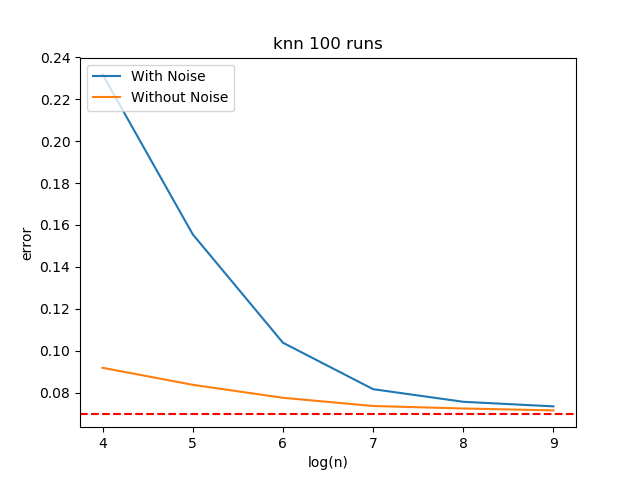
\includegraphics[width = 3.1in]{knn_100runs.png}} &
\subfloat[]{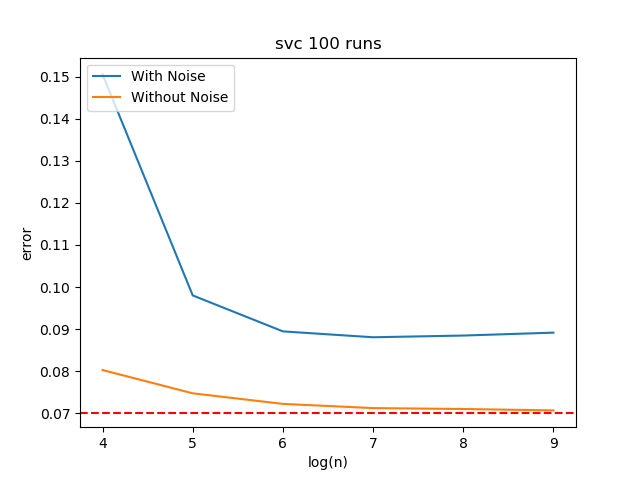
\includegraphics[width = 3.1in]{svc_100runs.png}} \\
\subfloat[]{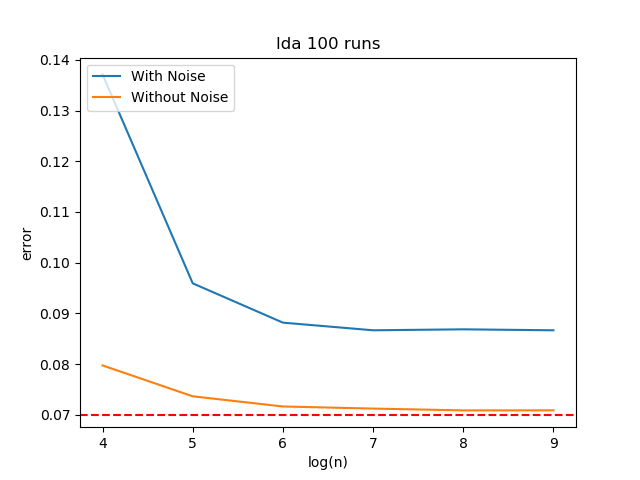
\includegraphics[width = 3.1in]{lda_100runs.png}} &
\subfloat[]{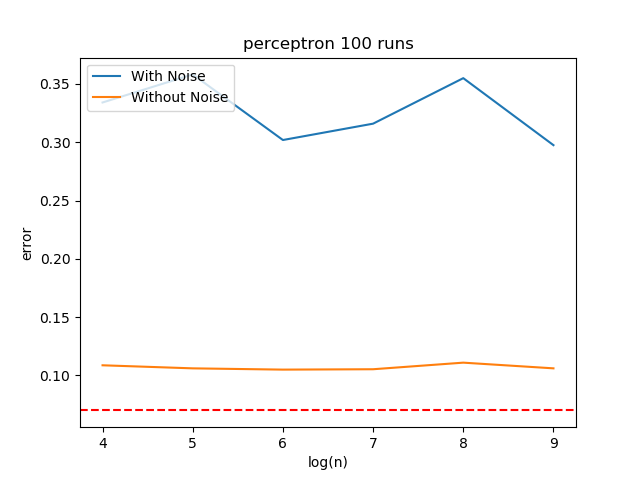
\includegraphics[width = 3.1in]{perceptron_100runs.png}}

\end{tabular}
\caption{Reproduced results from \cite{cannings2018classification} with data generated from multivariate Gaussian \& Perceptron Findings}
\end{figure*}

\subsection{Consistency in Perceptron and Deep Neural Networks}
\label{sec-5-2}

\begin{figure*}[!htp]
  % Maximum length
\subfloat[Prediction contour of Perceptron without Sigmoid activation]{\label{percep_w_sig}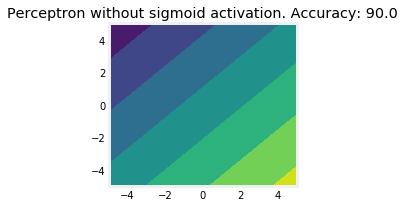
\includegraphics[height=3cm]{simple_models/percep_without_sigmoid.png}}\hfill
\subfloat[Prediction contour of Perceptron without Sigmoid activation]{\label{percep_sig}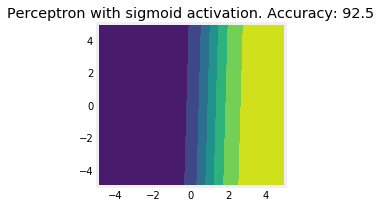
\includegraphics[height=3cm]{simple_models/percep_with_sigmoid.png}}\hfill
\subfloat[Prediction contour of Single Hidden Layer Neural Network without Sigmoid activation]{\label{simple_nn}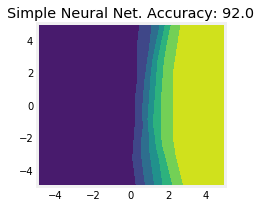
\includegraphics[height=3cm]{simple_models/simple_neural_net.png}}
   \caption{Analysis of Consistency of Perceptron with noisy data}
\end{figure*}


\begin{figure*}[!htp]
  % Maximum length
  \subfloat[Training losses of the different instances of the simple neural network]{\label{fig2:a}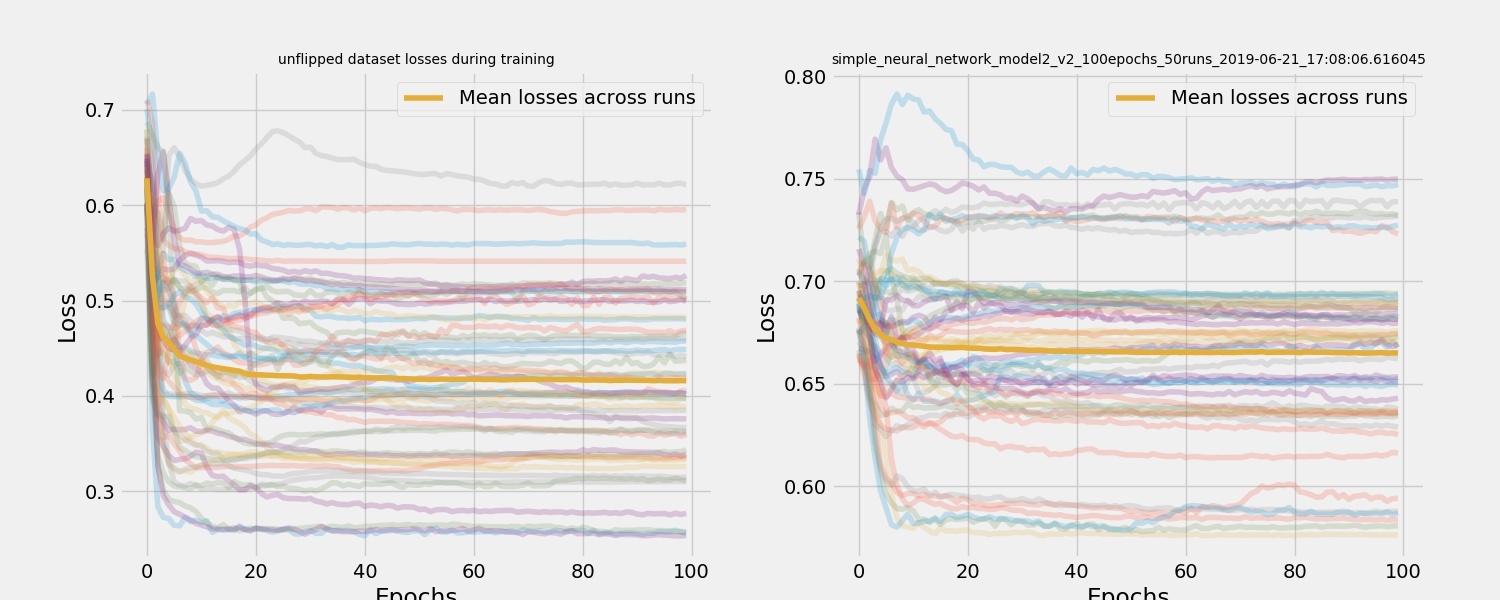
\includegraphics[width=1.00\linewidth]{NN_consistency/losses.jpg}}\\
  \subfloat[Average error rates of the samples trained single hidden layer neural networks.]{\label{fig2:b}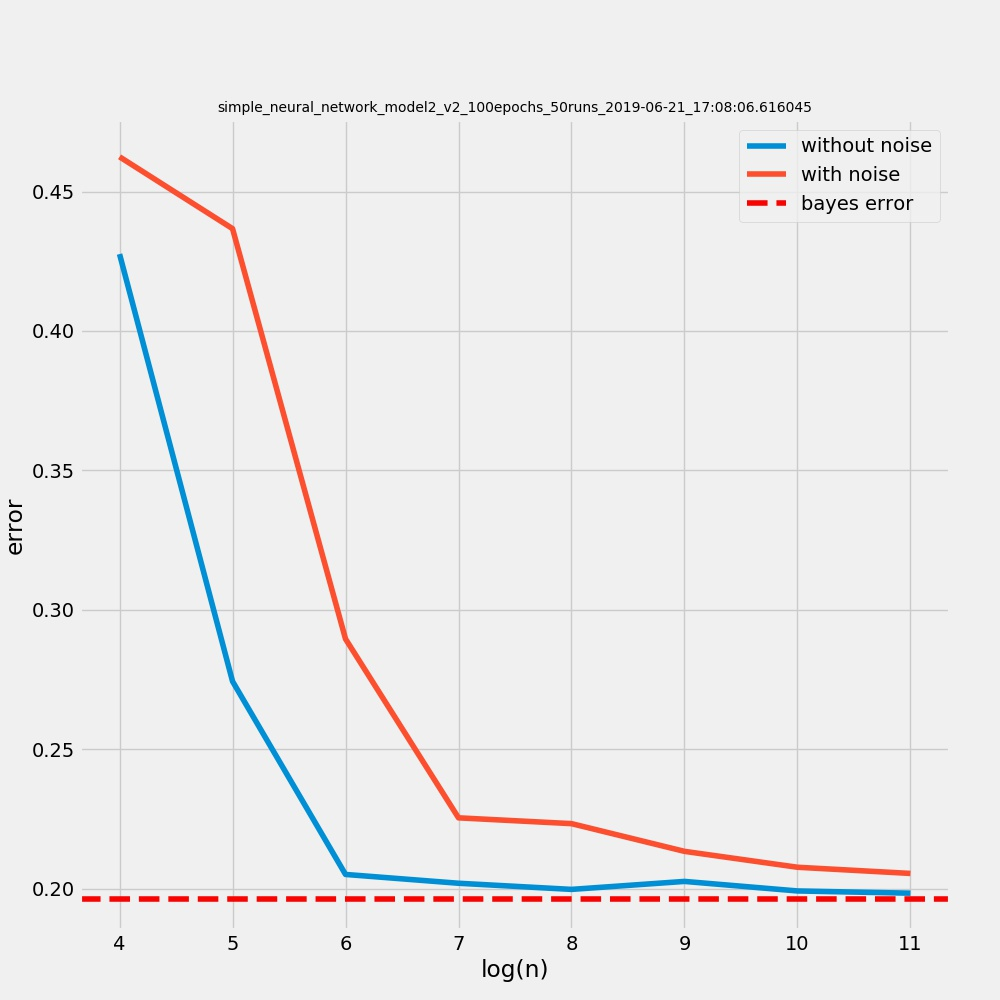
\includegraphics[width=0.33\linewidth]{NN_consistency/errors.jpg}}\hfill
  \subfloat[Prediction contour of trained neural network with original data.(without noise)]{\label{fig2:c}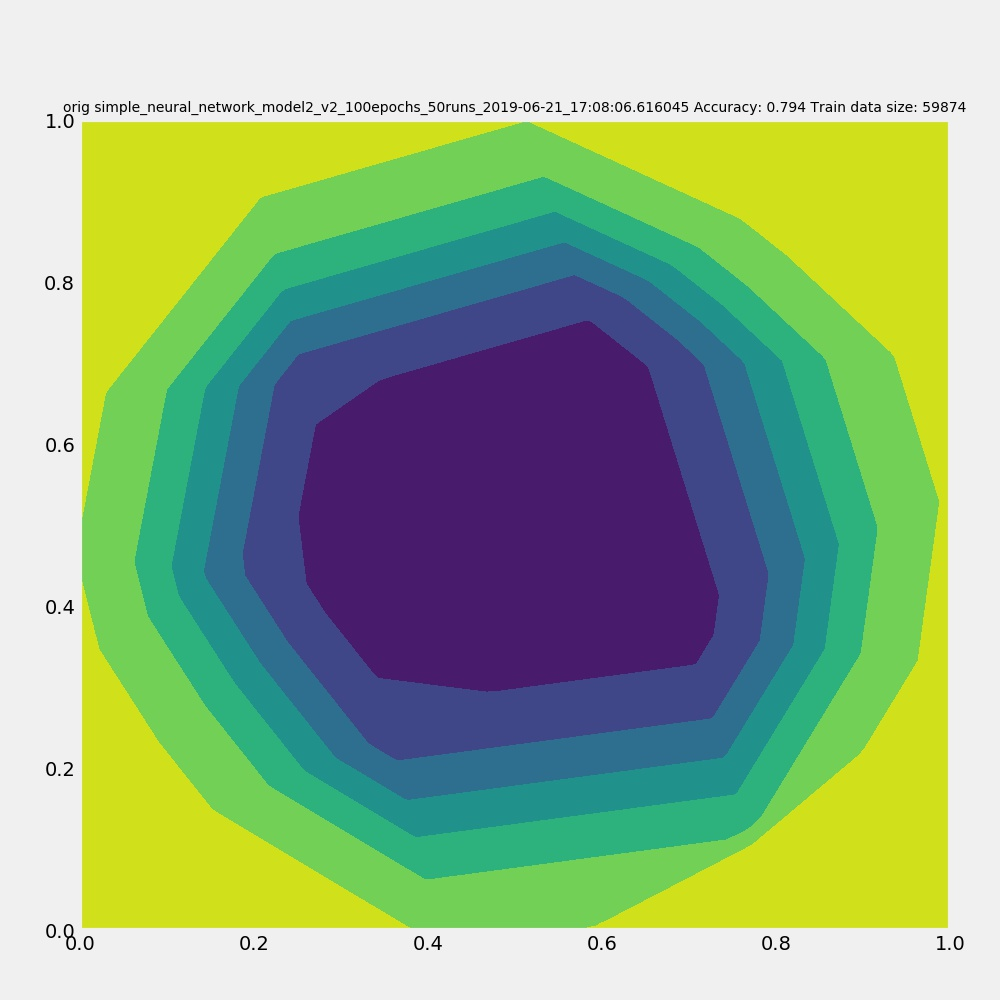
\includegraphics[width=0.33\linewidth]{NN_consistency/orig_simple_neural_network_model2_contour.jpg}}\hfill
  \subfloat[Prediction contour of trained neural network with original data.(without noise)]{\label{fig2:d}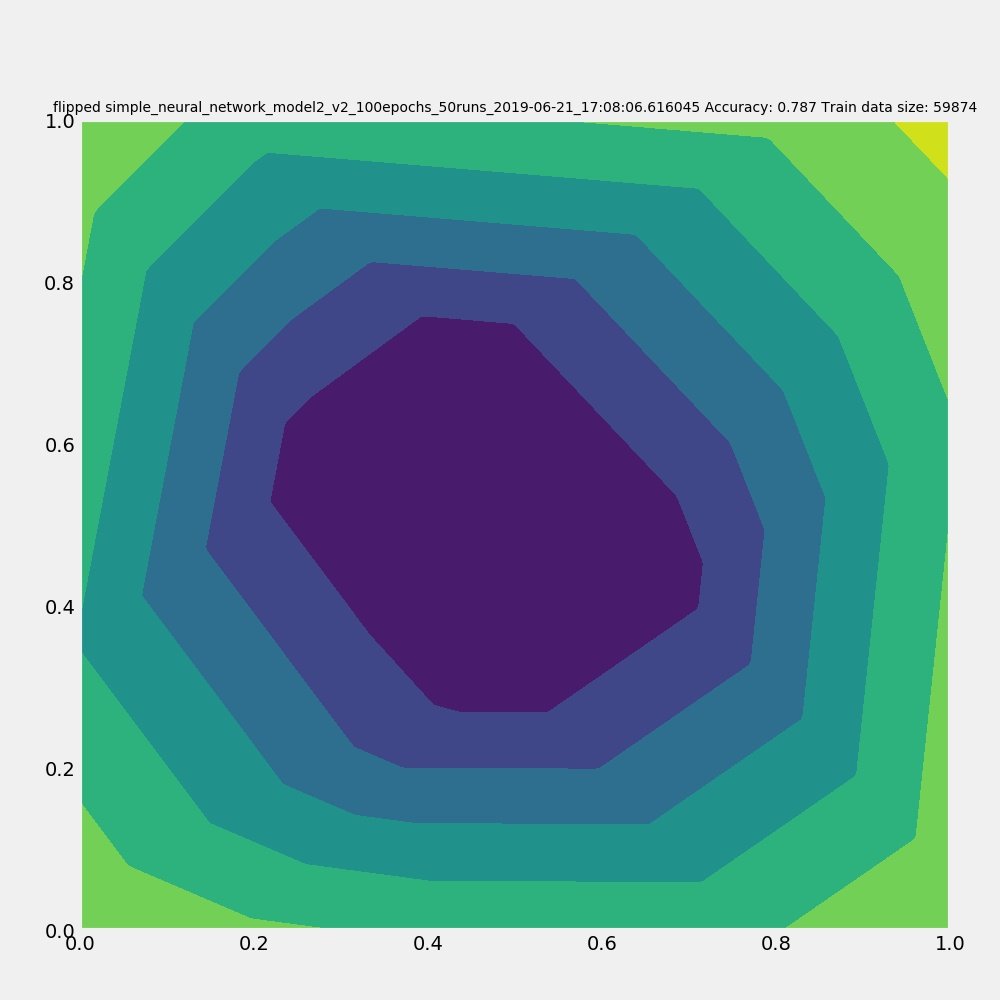
\includegraphics[width=0.33\linewidth]{NN_consistency/flipped_simple_neural_network_model2_contour.jpg}}
   \caption{Analysis of Consistency of Neural Networks with noisy data}
\end{figure*}



\subsection{Analysis of binary two-moons dataset classification using Bayesian Neural Networks(PyMC3)}
\label{sec-5-3}
\begin{figure*}[!htp]
    \subfloat[Toy Two Moon Dataset]{\label{2moondataset}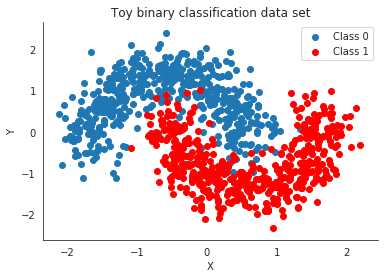
\includegraphics[width=0.50\linewidth]{bnn_classification_two_moon/dataset.png}}\hfill
    \subfloat[Prediction of Test Set by the Bayesian-NN  ]{\label{2moonpredicted}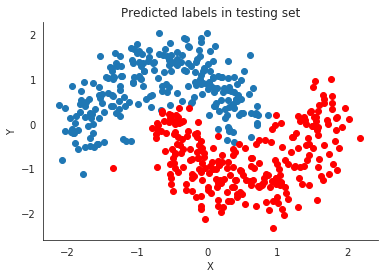
\includegraphics[width=0.50\linewidth]{bnn_classification_two_moon/predicted.png}}\\
    \subfloat[Prediction Contour]{\label{2moon_pred_contour}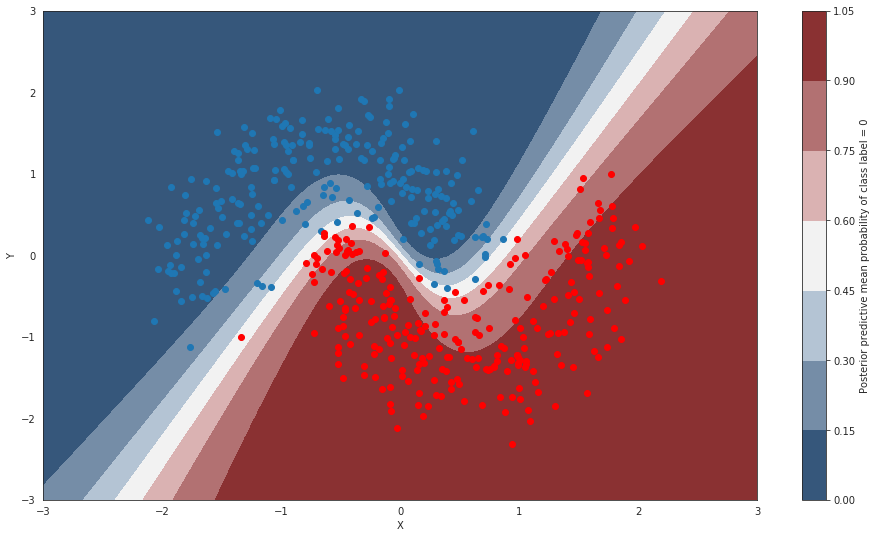
\includegraphics[width=0.50\linewidth]{bnn_classification_two_moon/prediction_contour.png}}\hfill
    \subfloat[Uncertainty Contour]{\label{2moon_uncer_contour}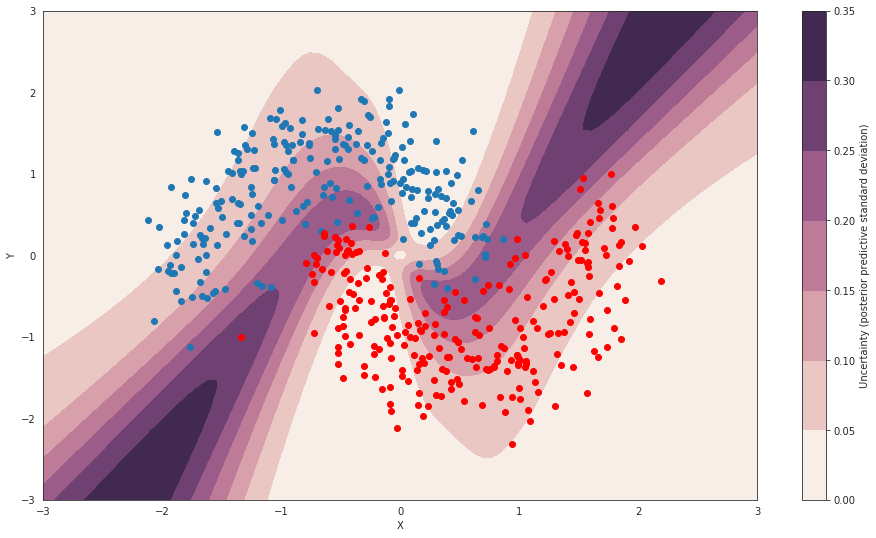
\includegraphics[width=0.50\linewidth]{bnn_classification_two_moon/uncertainity_contour.png}}\\
    \caption{Bayesian Neural Network trained to classify Two-Moon Dataset}
\end{figure*}



\subsection{Analysis of discontinuous regression using Bayesian Neural Networks(numpyro)}
\label{sec-5-4}

\begin{figure*}[!htp]
    \subfloat[sigma: 0.2 ]{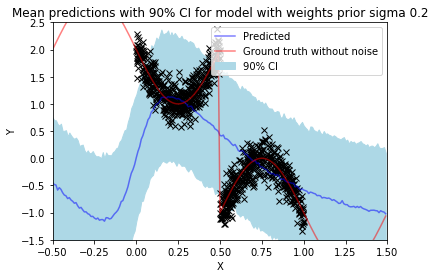
\includegraphics[width=0.20\linewidth]{discontinuous_regression/discont_reg_02.png}}\hfill
    \subfloat[sigma: 0.5 ]{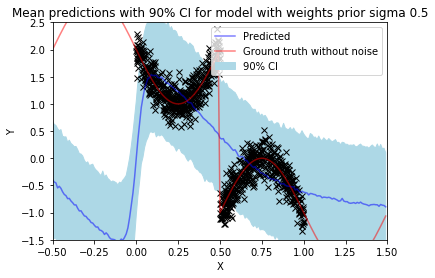
\includegraphics[width=0.20\linewidth]{discontinuous_regression/discont_reg_05.png}}\hfill
    \subfloat[sigma: 1.0 ]{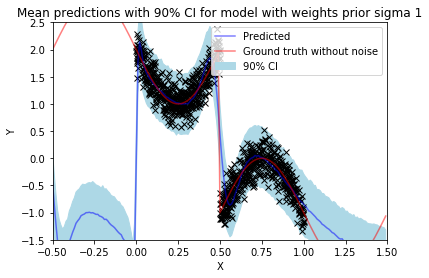
\includegraphics[width=0.20\linewidth]{discontinuous_regression/discont_reg_10.png}}\hfill
    \subfloat[sigma: 2.0 ]{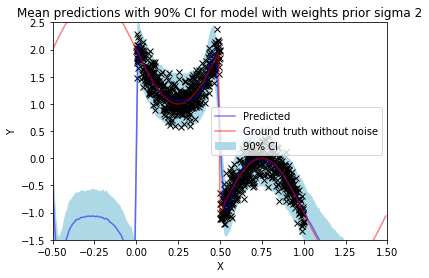
\includegraphics[width=0.20\linewidth]{discontinuous_regression/discont_reg_20.png}}\hfill
    \subfloat[sigma: 5.0 ]{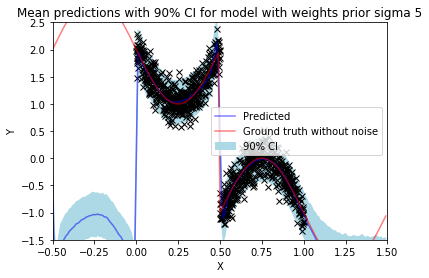
\includegraphics[width=0.20\linewidth]{discontinuous_regression/discont_reg_50.png}}\\
    \subfloat[Box plot of effective sample size of weights of each layer]{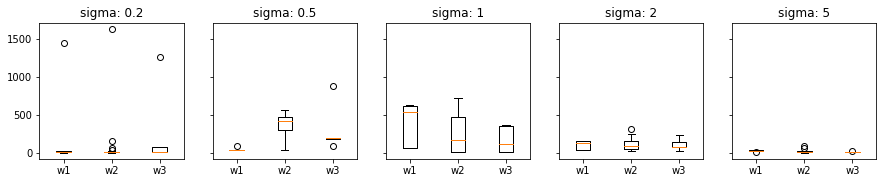
\includegraphics[width=1.00\linewidth]{discontinuous_regression/discont_effective_samples.png}}\\
    \caption{Discontinuous regression using Bayesian Neural Networks}
\end{figure*}


\subsection{Analysis of continuous regression using Bayesian Neural Networks(numpyro)}
\label{sec-5-5}

\begin{figure*}[!htp]
    \subfloat[sigma: 0.2 ]{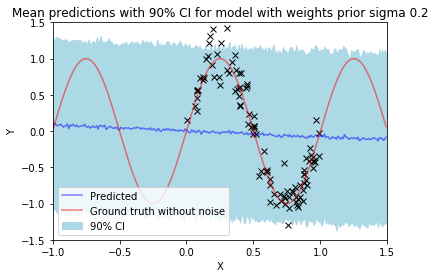
\includegraphics[width=0.20\linewidth]{continuous_regression/cont_reg_02.png}}\hfill
    \subfloat[sigma: 0.5 ]{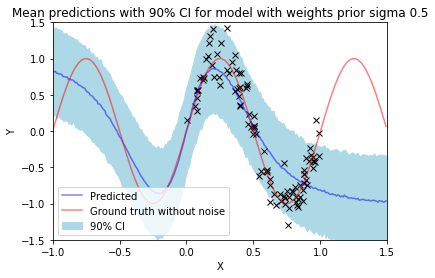
\includegraphics[width=0.20\linewidth]{continuous_regression/cont_reg_05.png}}\hfill
    \subfloat[sigma: 1.0 ]{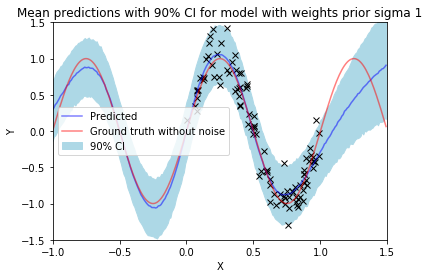
\includegraphics[width=0.20\linewidth]{continuous_regression/cont_reg_10.png}}\hfill
    \subfloat[sigma: 2.0 ]{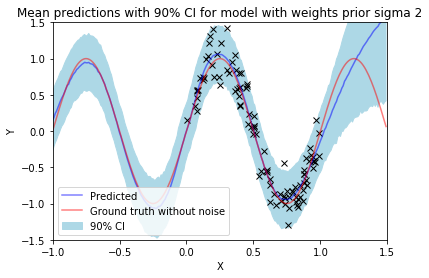
\includegraphics[width=0.20\linewidth]{continuous_regression/cont_reg_20.png}}\hfill
    \subfloat[sigma: 5.0 ]{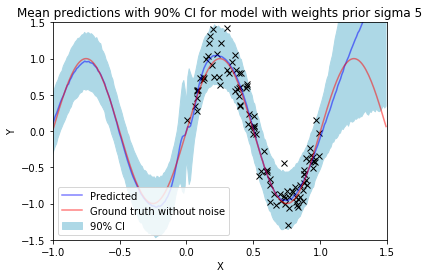
\includegraphics[width=0.20\linewidth]{continuous_regression/cont_reg_50.png}}\\
    \subfloat[Box plot of effective sample size of weights of each layer]{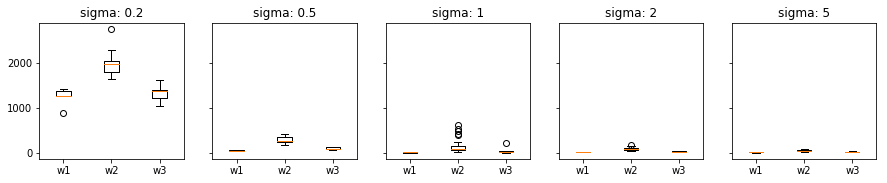
\includegraphics[width=1.00\linewidth]{continuous_regression/cont_effective_samples.png}}\\
    \caption{Continuous regression using Bayesian Neural Networks}
\end{figure*}


\section{Conclusion}
\label{sec-6}

\section{Future Work}
\label{sec-7}
% Emacs 25.2.2 (Org mode 8.2.10)
\end{document}